\section{Ejercicio 2}

\subsection{Introducción}

\paragraph{}
En esta sección se presentara un algoritmo exacto para resolver el problema de encontrar la Clique Máxima en un grafo.

\paragraph{}
Aún no se conocen algoritmos buenos, es decir, polinomiales con respecto al tamaño de la entrada para resolver 
este problema. Así que nos consentraremos en realizar mejoras al algoritmo de fuerza bruta que considera todos los casos.


\subsection{Explicación}
\label{explicacion2}
\paragraph{}
Un algoritmo de fuerza bruta para resolver el problema de Max-Clique podría simplemente intentar formar el conjunto más 
grande de nodos, donde ese conjunto sea completo, intentando todas las posibilidades eligiendo todos los conjuntos de un cierto tamaño,
luego intentar con un tamaño menor, etc. Probablemente la complejidad de un algoritmo de este estilo sea $n^n$ donde n es la cantidad 
de nodos del grafo.

\paragraph{}
Una mejora que surge casi inmediatamente es utilizar la técnica de BackTracking, cuya función principal es intentar podar el 
arbol implicito de combinaciones posibles. 

\paragraph{}
De todas maneras, implementar solo un BackTracking parece ser poco con respecto a las mejoras que se pueden lograr. A continuación, se explicara el algoritmo implementado con algunas mejoras, su pseudocodigo, y se verá cada una de las mejoras por separado.

\vspace{2em}
\incmargin{3em}
\linesnumbered
\restylealgo{boxed}
\footnotesize 
\textbf{Algoritmo Exacto}(G: grafo) \\
\begin{algorithm}[H]
	\BlankLine
		CliqueMayor = vacia\\
		componentesConexas = DetectarComponentesConexas(G)
		\BlankLine

		\textbf{Para cada} componente \textbf{en} componentesConexas \{ 
		\BlankLine

		\tab\tab heap = crearHeap(G,componentes) \\

		\BlankLine
		\tab\tab \textbf{Mientras} noVacio(heap) $\wedge$ top(heap) $\geq$ tam(CliqueMayorActual)\{\\
		\BlankLine
		\tab\tab\tab v = top(heap)
		\BlankLine
		\tab\tab\tab \textbf{Para} tamCliqueABuscar \textbf{desde} grado(v)+1 \textbf{hasta} tam(CliqueMayorActual)+1\{\\
		\tab\tab\tab\tab vecinosFiltrados = 	filtrarVecinosMenores(v, tamCliqueABuscar-1)\\						
		\tab\tab\tab\tab \textbf{Si} tam(vecinosFiltrados) +1 $\geq$ tamCliqueABuscar\\ 			
		\tab\tab\tab\tab\tab temp = BuscoCliqueDeTamañoK(tamCliqueABuscar, vecinosFiltrados)
		\BlankLine
		\tab\tab\tab\tab\tab \textbf{Si}  tam(CliqueMayorActual)  $<$ tam(temp)\\ 
		\tab\tab\tab\tab\tab\tab CliqueMayorActual  = temp\\
		\tab\tab\tab\}\\
		\tab\tab\}
\caption{Pseudocódigo del algoritmo exacto}
\end{algorithm}

\normalsize

\paragraph{}
Primero, se detectan las componentes conexas del grafo, ya que buscar la max clique en todo el grafo es equivalente a quedarse con la máxima de las max cliques de cada componente conexa.

\paragraph{}
Luego, para cada componente, se crea un heap que contiene los nodos de la componente ordenados por mayor grado. Esto no parece tener mucha importancia, pero se aclarará a medida que se avanza con la explicación.

\paragraph{}
A partir de esta estructura, vamos obteniendo en cada iteración, el nodo $v$ de mayor grado disponible en la componente que no hayamos analizado.

\paragraph{}
Una vez que tenemos el nodo $v$, lo que se hace es buscar la mayor clique en la cual está contenido. Para ello utilizamos la función BuscoCliqueDeTamañoK a la cual le indicamos el tamaño de la clique que queremos buscar (desde el grado de $v$ + 1) y los vecinos de $v$ que, dado su grado, tienen posibilidades de pertenecer a la clique.

\paragraph{}
Por ejemplo, veamos la siguiente figura:

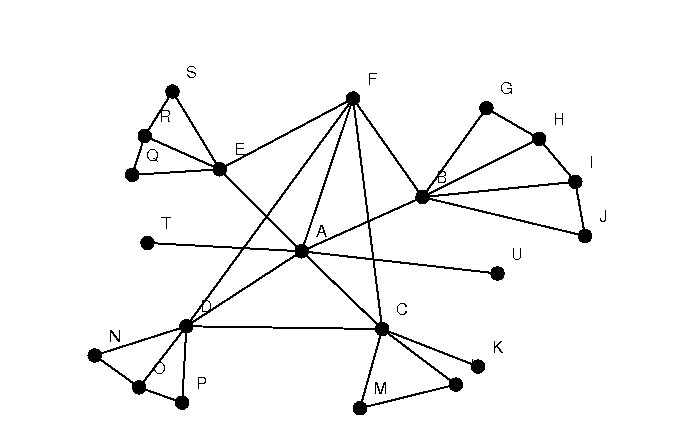
\includegraphics[scale = 0.9]{./otros/p.jpg} \\

\paragraph{}
Como se ve en el ejemplo, si buscamos cliques que contengan al vertice A (cuyo grado es 7), no tendria sentido buscarlas de cualquier tamaño, sino desde el grado del vertice más uno, es decir, cliques de tamaño 8 en este caso. Pero si vemos cuantos nodos vecinos de grado 7 tiene, notamos que no alcanzan para formar una clique de 8. Luego buscamos nodos vecinos de A de grado 6 o más y notamos que hay 3 (B, C, D) y A, por lo tanto tampoco alcanzan para una clique de tamaño 7. Luego los de grado 5 o más, encontramos 5 más A. En este caso, hay probabilidades de que estos 6 nodos puedan formar una clique de tamaño 6, entonces realizaremos una busqueda exaustiva utilizando backtracking, el cual en este caso dara negativo ya que no hay cliques de grado 6 en el grafo que contengan a A. Una vez más, buscaremos una clique de tamaño 5, para lo cual solo miraremos nodos de grado 4 o más y realizaremos el backtracking sobre los nodos disponibles. 

\paragraph{}
De todas maneras, el algoritmo intentará buscar cliques cada vez mas chicas hasta llegar a cliques de del tamaño de la más grande encontrada hasta el momento (sin incluir). Esto es así puesto que no tiene sentdo seguir buscando cliques más chicas que la mayor encontrada hasta el momento. 

\paragraph{}
El heap de nodos ordenados por grados tiene gran importancia, ya que permite decidir rapidamente cuando terminar con la busqueda. Esto se realiza comprobando que el nodo siguiente del heap, es decir, el de mayor grado de la componente, supere o iguale al tamaño de la clique mas grande encontrada, ya que en caso contrario, no tendría sentido seguir buscando dentro de esa clique.
\clearpage

\newpage

\subsection{Resultados}

\paragraph{}
A continuación se presentan los gráficos provenientes de las pruebas realizadas con archivos generados al azar. La forma en la que fueron generados estos archivos de entrada es explicada en la sección [\ref{anexo}].
%primeras 2 imagenes
\begin{figure}[h]
    \begin{minipage}{\textwidth}
	\begin{center}
		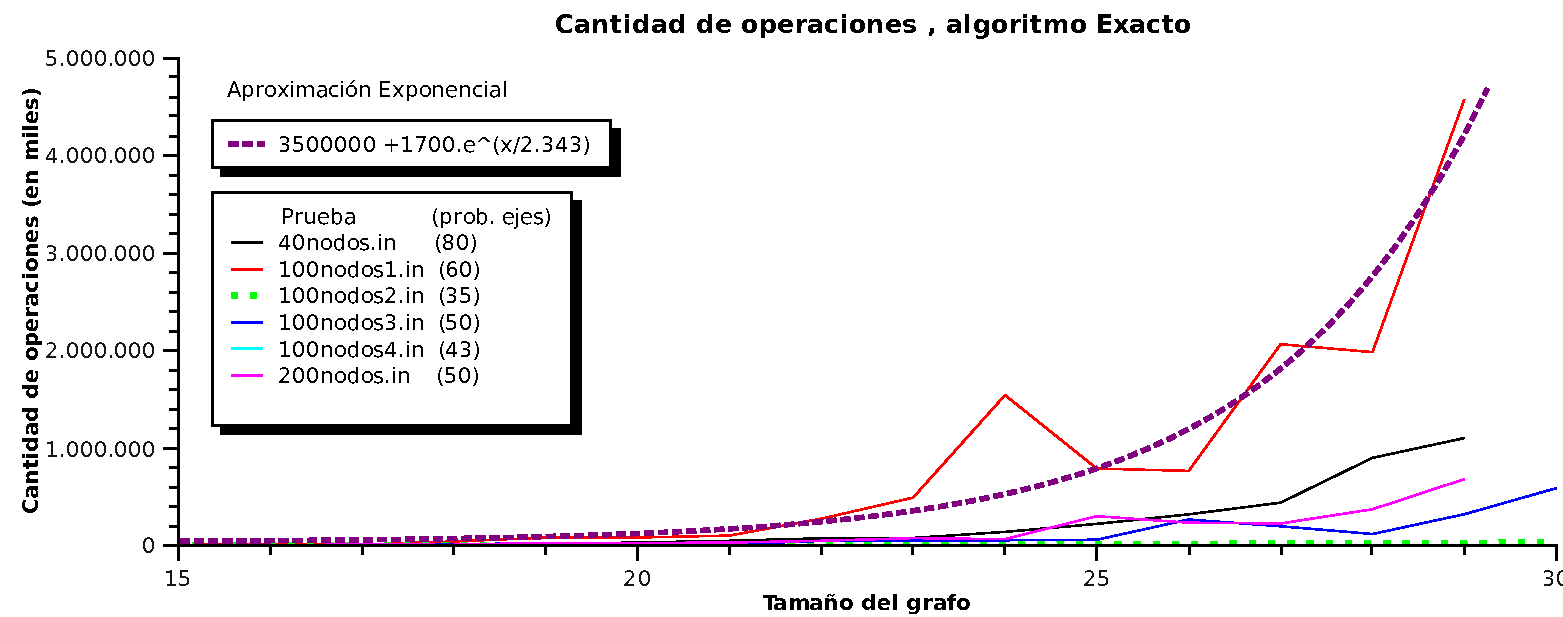
\includegraphics[width=\textwidth]{./otros/graficos/operaciones_ej2.pdf}
		\caption{Muestra el comportamiento del algoritmo exacto, comparando el rendimiento del algoritmo para distintas cantidades de nodos contra cantidad de operaciones realizadas efectivamente. La probabilidad de aparición de ejes en estas muestras fueron las presentes en la tabla entre paréntesis. También, aparece una función exponencial generada con qti plot en base a los datos de la tabla que aproxima una de las mediciónes (100nodos1.in en este caso).}
		\label{ej2contarOp}
	\end{center}
    \end{minipage}

\end{figure}


\begin{figure}[h]
    \begin{minipage}{\textwidth}
	\begin{center}
		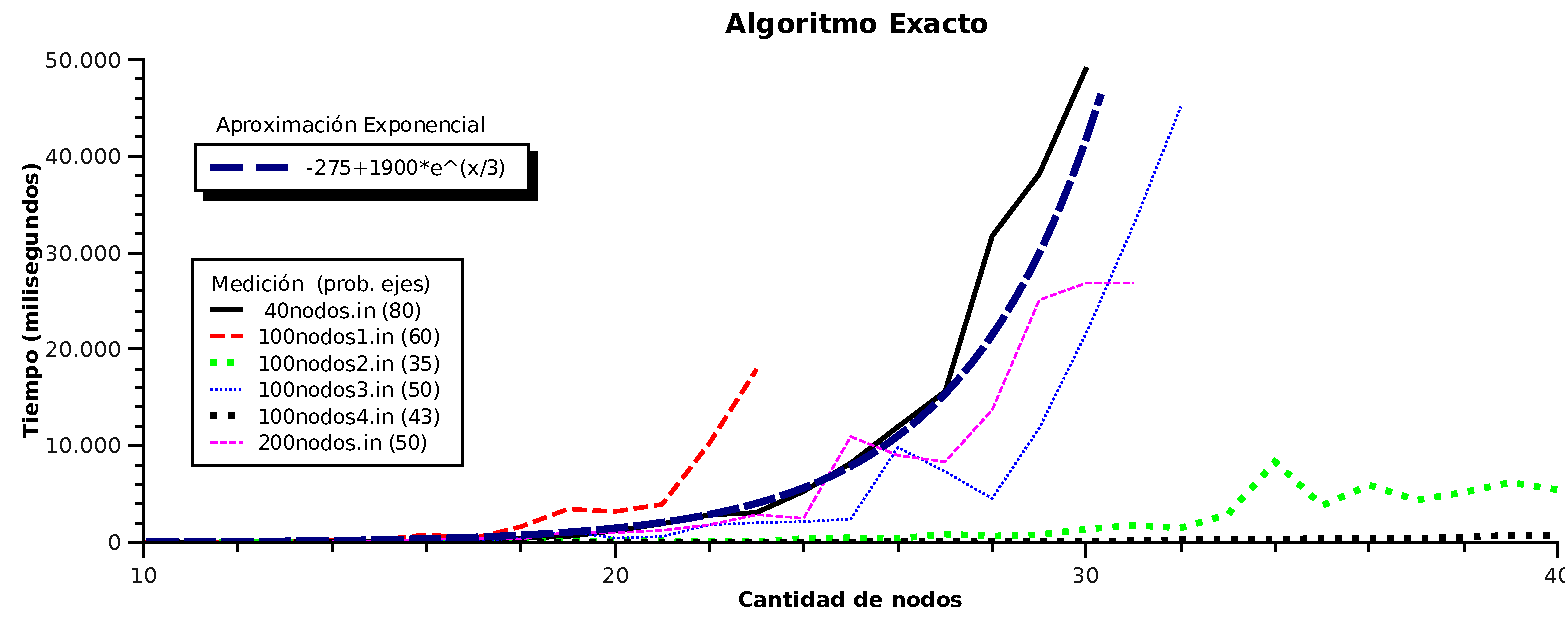
\includegraphics[width=\textwidth]{./otros/graficos/tiempo_ej2.pdf}
		\caption{Muestra el comportamiento del algoritmo exacto, comparando el rendimiento del algoritmo para distintas cantidades de nodos contra el tiempo que demoro en devolver los resultados. La probabilidad de aparición de ejes en estas muestras fueron las presentes en la tabla entre paréntesis. También, aparece una función exponencial generada con qti plot en base a los datos de la tabla que aproxima una de las mediciónes (40nodos.in en este caso)}
		\label{ej2contarTiempo}
	\end{center}
    \end{minipage}

\end{figure}


\subsection{Debate y conclusiones}
\paragraph{}
Viendo los gráficos podemos ver que para estos casos, el algoritmo se comporto como se esperaba (Exponencialmente) salvo algunos casos donde pareciera estar acotados por alguna función polinomica. Sin embargo en general esto no ocurre.

\paragraph{}
La única diferencia notable entre distintas pruebas fue que en los casos de prueba en los que había más ejes, es decir, en aquellos casos en que los grafos eran más densos, el algoritmo empeora, excepteptuando casos donde el grafo era muy denso (superior al 80\% de los ejes presentes) en cuyo caso funciona un poco mejor por lo explicado en la sección [\ref{explicacion2}].

\paragraph{}
Podemos concluir entonces que suponer que el algoritmo exacto no es bueno, es decir, es exponencial, era correcto.




